\chapter{Differentiating Through the Forward Solver}\label{ch:adjoint}

Computing the gradient $\nabla_\phi \ell$ of the
log-likelihood~\cref{eq:log-likelihood} requires differentiating through
the forward map~$\mathcal{P}$, which involves solving a sequence of
tridiagonal linear systems. In this chapter we derive an efficient adjoint
method for this computation, demonstrate its value through gradient-based
optimisation, and compare against a gradient-free alternative.

\section{Discretise Then Optimise}\label{sec:disc-then-opt}

There are two strategies for differentiating through a numerical solver.
The \emph{optimise then discretise} approach derives continuous adjoint
equations and then discretises them; the \emph{discretise then optimise}
approach differentiates the discrete computation directly. We adopt the
latter, which yields the exact gradient of the quantity evaluated in code
and avoids consistency errors between the forward and adjoint
discretisations~\cite{kidger2021neural}.

\section{Reverse-Mode AD and the Cost of Na\"ive Taping}%
\label{sec:reverse-ad}

Since $\ell$ is scalar-valued, reverse-mode automatic differentiation
(AD) computes the full gradient in a single backward pass regardless of
the number of parameters. Reverse-mode AD decomposes the computation into
a sequence of \emph{vector--Jacobian products} (VJPs): if the forward
computation is $f = f_L \circ \cdots \circ f_1$, the chain rule gives
\begin{equation}
  \frac{\partial f}{\partial \phi}
  = J_{f_L}\, J_{f_{L-1}} \cdots J_{f_1},
  \label{eq:chain-rule}
\end{equation}
which reverse mode evaluates from left to right, multiplying the adjoint
(cotangent) vector by each Jacobian in turn without forming the
intermediate matrices explicitly. The dominant primitives in
$\mathcal{P}$ are the $m$ tridiagonal solves, so the central question is
how to implement the VJP of a single solve $Ax = b$.

A generic AD framework will tape every intermediate scalar of the Thomas
algorithm -- elimination multipliers, modified diagonals, partial sums
-- and replay them in reverse. Since the tape must be retained across
all $m$ timesteps, the total memory scales as $O(mn)$ with a large
per-timestep constant, and the overhead of maintaining and traversing
the tape degrades runtime even when memory is not the binding constraint.

\section{Adjoint of the Tridiagonal Solve}\label{sec:adjoint-solve}

We avoid taping by exploiting the structure of the linear solve.
Suppose the forward pass solves $Ax = b$ and the backward pass receives
the adjoint $\bar{x} = \partial \ell / \partial x$. The adjoint with
respect to $b$ is
\begin{equation}
  \bar{b}
  = \bar{x}^T \frac{\partial x}{\partial b}
  = \bar{x}^T A^{-1},
  \label{eq:adjoint-b}
\end{equation}
which is equivalent to solving the \emph{adjoint system}
\begin{equation}
  A^T \lambda = \bar{x}
  \label{eq:adjoint-system}
\end{equation}
and setting $\bar{b} = \lambda^T$. For the matrix adjoint, we
differentiate the identity $Ax = b$:
\begin{equation}
  dA\, x + A\, dx = db.
\end{equation}
Left-multiplying by $\lambda^T$ and using $\lambda^T A = \bar{x}^T$
gives $\lambda^T dA\, x + \bar{x}^T dx = \lambda^T db$. Since
$\bar{x}^T dx$ contributes to $\bar{b}$, the
adjoint with respect to $A$ is
\begin{equation}
  \bar{A} = -\lambda\, x^T,
  \label{eq:adjoint-A}
\end{equation}
where $\bar{A}_{ij} = -\lambda_i\, x_j$.

The key observation is that $A^T$ is also tridiagonal, so the adjoint
system~\cref{eq:adjoint-system} is solved by the Thomas algorithm at the
same $O(n)$ cost as the forward solve. Only the matrix $A$ diagonals and the
forward solution $x$ need to be cached per timestep -- four arrays of
length $n$, rather than the full tape of Thomas algorithm intermediates.

In practice we define a custom VJP rule in
JAX~\cite{jax2018github}: the forward pass solves $Ax = b$ and caches
$A$ and $x$; the backward pass solves $A^T \lambda = \bar{x}$ and
returns $\bar{b} = \lambda^T$ and $\bar{A} = -\lambda\, x^T$. No taping
of the Thomas algorithm's internal operations is required.

\subsection{Full Backward Pass}\label{sec:full-backward}

The custom VJP handles a single timestep. The full gradient
$\nabla_\phi \ell$ is assembled by walking backward through time levels
$k = m, m-1, \ldots, 1$. At each level the adjoint
system~\cref{eq:adjoint-system} is solved using the cached $A^k$
and~$x^k$, yielding $\lambda^k$ and the matrix adjoint
$\bar{A}^k = -\lambda^k (x^k)^T$. Only the first row of $A^k$ depends
on $\phi$ (through the Butler--Volmer coefficients $K_{\mathrm{red}}$
and $K_{\mathrm{ox}}$; the interior rows are parameter-independent), so
the contributions to $\nabla_\phi \ell$ come exclusively from $\bar{A}^k$
applied to the partial derivatives $\partial A^k_{0,\cdot} / \partial
\phi$, which are accumulated across timesteps. The result is the exact
gradient of the discrete log-likelihood at a cost of one adjoint solve
per timestep.

\section{Extension to Pentadiagonal Systems}\label{sec:pentadiagonal}

The adjoint generalises directly to pentadiagonal systems: the transpose
of a pentadiagonal matrix is again pentadiagonal, so the adjoint system
is solved at the same $O(n)$ cost per timestep. The saving over na\"ive
taping grows with bandwidth, since a pentadiagonal factorisation produces
more intermediates. We exploit this in
\cref{ch:heterogeneous,ch:adsorption}, where coupled multi-species
reactions lead to pentadiagonal structure.

\section{Optimisation Results}\label{sec:init-results}

We now use the adjoint gradient to locate the posterior mode before
sampling, eliminating the burn-in waste observed in
\cref{sec:sampling-results}. We compare the gradient-based ADAM
optimiser~\cite{kingma2014adam,deepmind2020jax} against
CMA-ES~\cite{hansen2001evolution,evosax2022github},
a gradient-free evolutionary strategy that adapts a population covariance
over generations. A single ADAM step (one forward and one adjoint solve)
costs approximately two forward-solve equivalents; one CMA-ES generation
costs $\lambda = 4 + \lfloor 3 \times \ln d\rfloor = 7$
\cite{hansen2001evolution}
forward solves. We equalise the total budget in forward-solve
equivalents so that both algorithms consume the same runtime.

\Cref{fig:electron-optim} shows the log-posterior density over the
course of optimisation at two noise levels ($\eta = 0.01$ and
$\eta = 0.02$), each run from $32$ initial conditions drawn using
Latin hypercube sampling centered at the true parameters. ADAM
reaches the high-density region in fewer
forward-solve equivalents and with lower variance across initialisations:
at $\eta = 0.02$, all $32$ runs are within $5\%$ of the modal
log-density by iteration $100$. Once ADAM reaches the mode it remains
stable, making it a suitable initialisation strategy for the MCMC
samplers. The difference between the performance of these
optimisation methods is not important in this problem -- we could use
CMA-ES to initialise the chains and obtain similar results -- but
this is not true when we increase the complexity of the problems. As
we will see in \cref{ch:heterogeneous,ch:adsorption}, the gradient
based optimisation becomes crucial to finding posterior modes efficiently.

\begin{figure}[ht]
  \begin{center}
    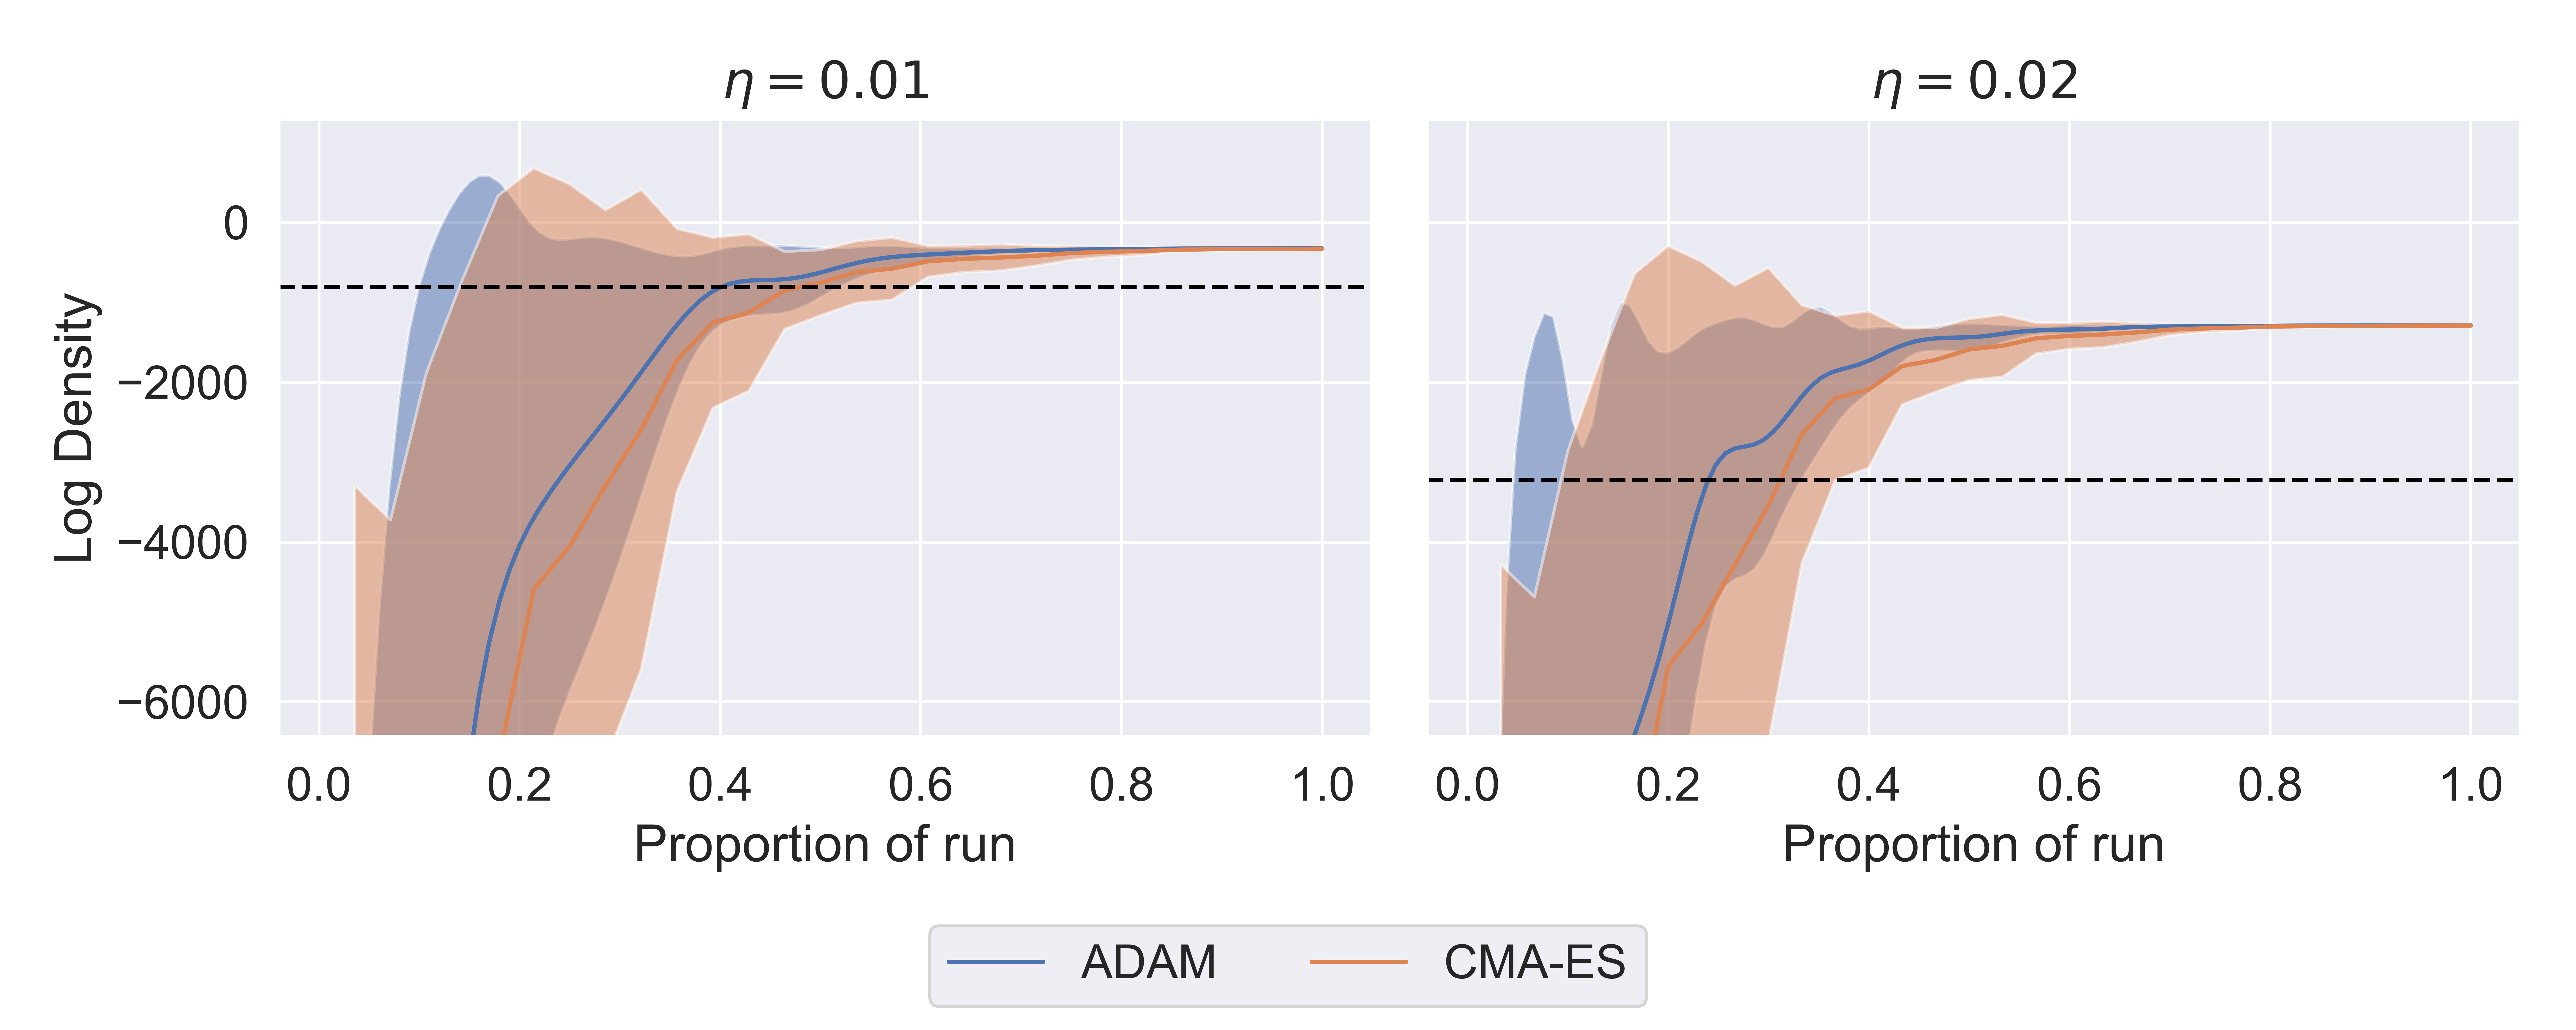
\includegraphics[width=0.95\textwidth]{figures/5-optim.png}
  \end{center}
  \caption[ADAM vs CMA-ES optimisation comparison]{Log-posterior density
    during optimisation for ADAM and CMA-ES (population size~$7$) at
    noise levels $\eta = 0.02$ and $\eta = 0.01$. Each algorithm is run
    from $32$~randomly drawn initial conditions; solid lines show the
    mean and shaded regions indicate $\pm 1$ standard deviation across
    runs. The black dashed line marks the two times the log-density
    evaluated at the true parameters~$\phi^*$ -- indicating high
    density regions. Both algorithms are given equal total
    computational budgets measured in forward-solve equivalents. 105
  steps for ADAM and 30 iterations for CMA-ES.}
  \label{fig:electron-optim}
\end{figure}
